\documentclass{article}
\usepackage{amsmath}
\usepackage{amssymb}
\usepackage{mathrsfs}
\usepackage{physics}
\usepackage{comment}
\usepackage{mathtools}
\newcommand{\om}{\omega_n}
\newcommand{\adag}{a^\dagger}
\newcommand{\s}{\item[]}
\newcommand\Chi{\mathrm{X}}
\newtheorem{problem}{Problem}
\title{Journal Two }
\author{Eesh Gupta}
\begin{document}
\maketitle






\begin{itemize}
\item \textbf{What has been the most significant challenge you have faced in the research environment? This could either be in your
research activities or in terms of personal and professional relationships.}
\begin{itemize}
  \s \textit{\textbf{Managing Autonomy}}:Having built a good relationship with my faculty mentor over
  the course of spring semester and now this summer, I have a greater
  control over
  designing experiments, selecting research papers for ``deep-reading'', and
  choosing which concepts to make a comprehensive report on. While
  my faculty mentor still guides me through the rough spots, the wheel
  is in my hands most of the times. Such autonomy, however, translates to an increased sense of
  pressure to produce ``progress''. And this can get overwhelming, especially when some experiment fails to produce meaningful results or when a topic
  becomes too hard to understand. However,
  having my Gandalf poster (Figure \ref{fig1}) on the opposite wall and ``the Avengers'' soundtrack buzzing
  in my room, I tell myself, ``Whatever it takes!'' And I get moving.
  \begin{figure}[!htb]
	\centering
	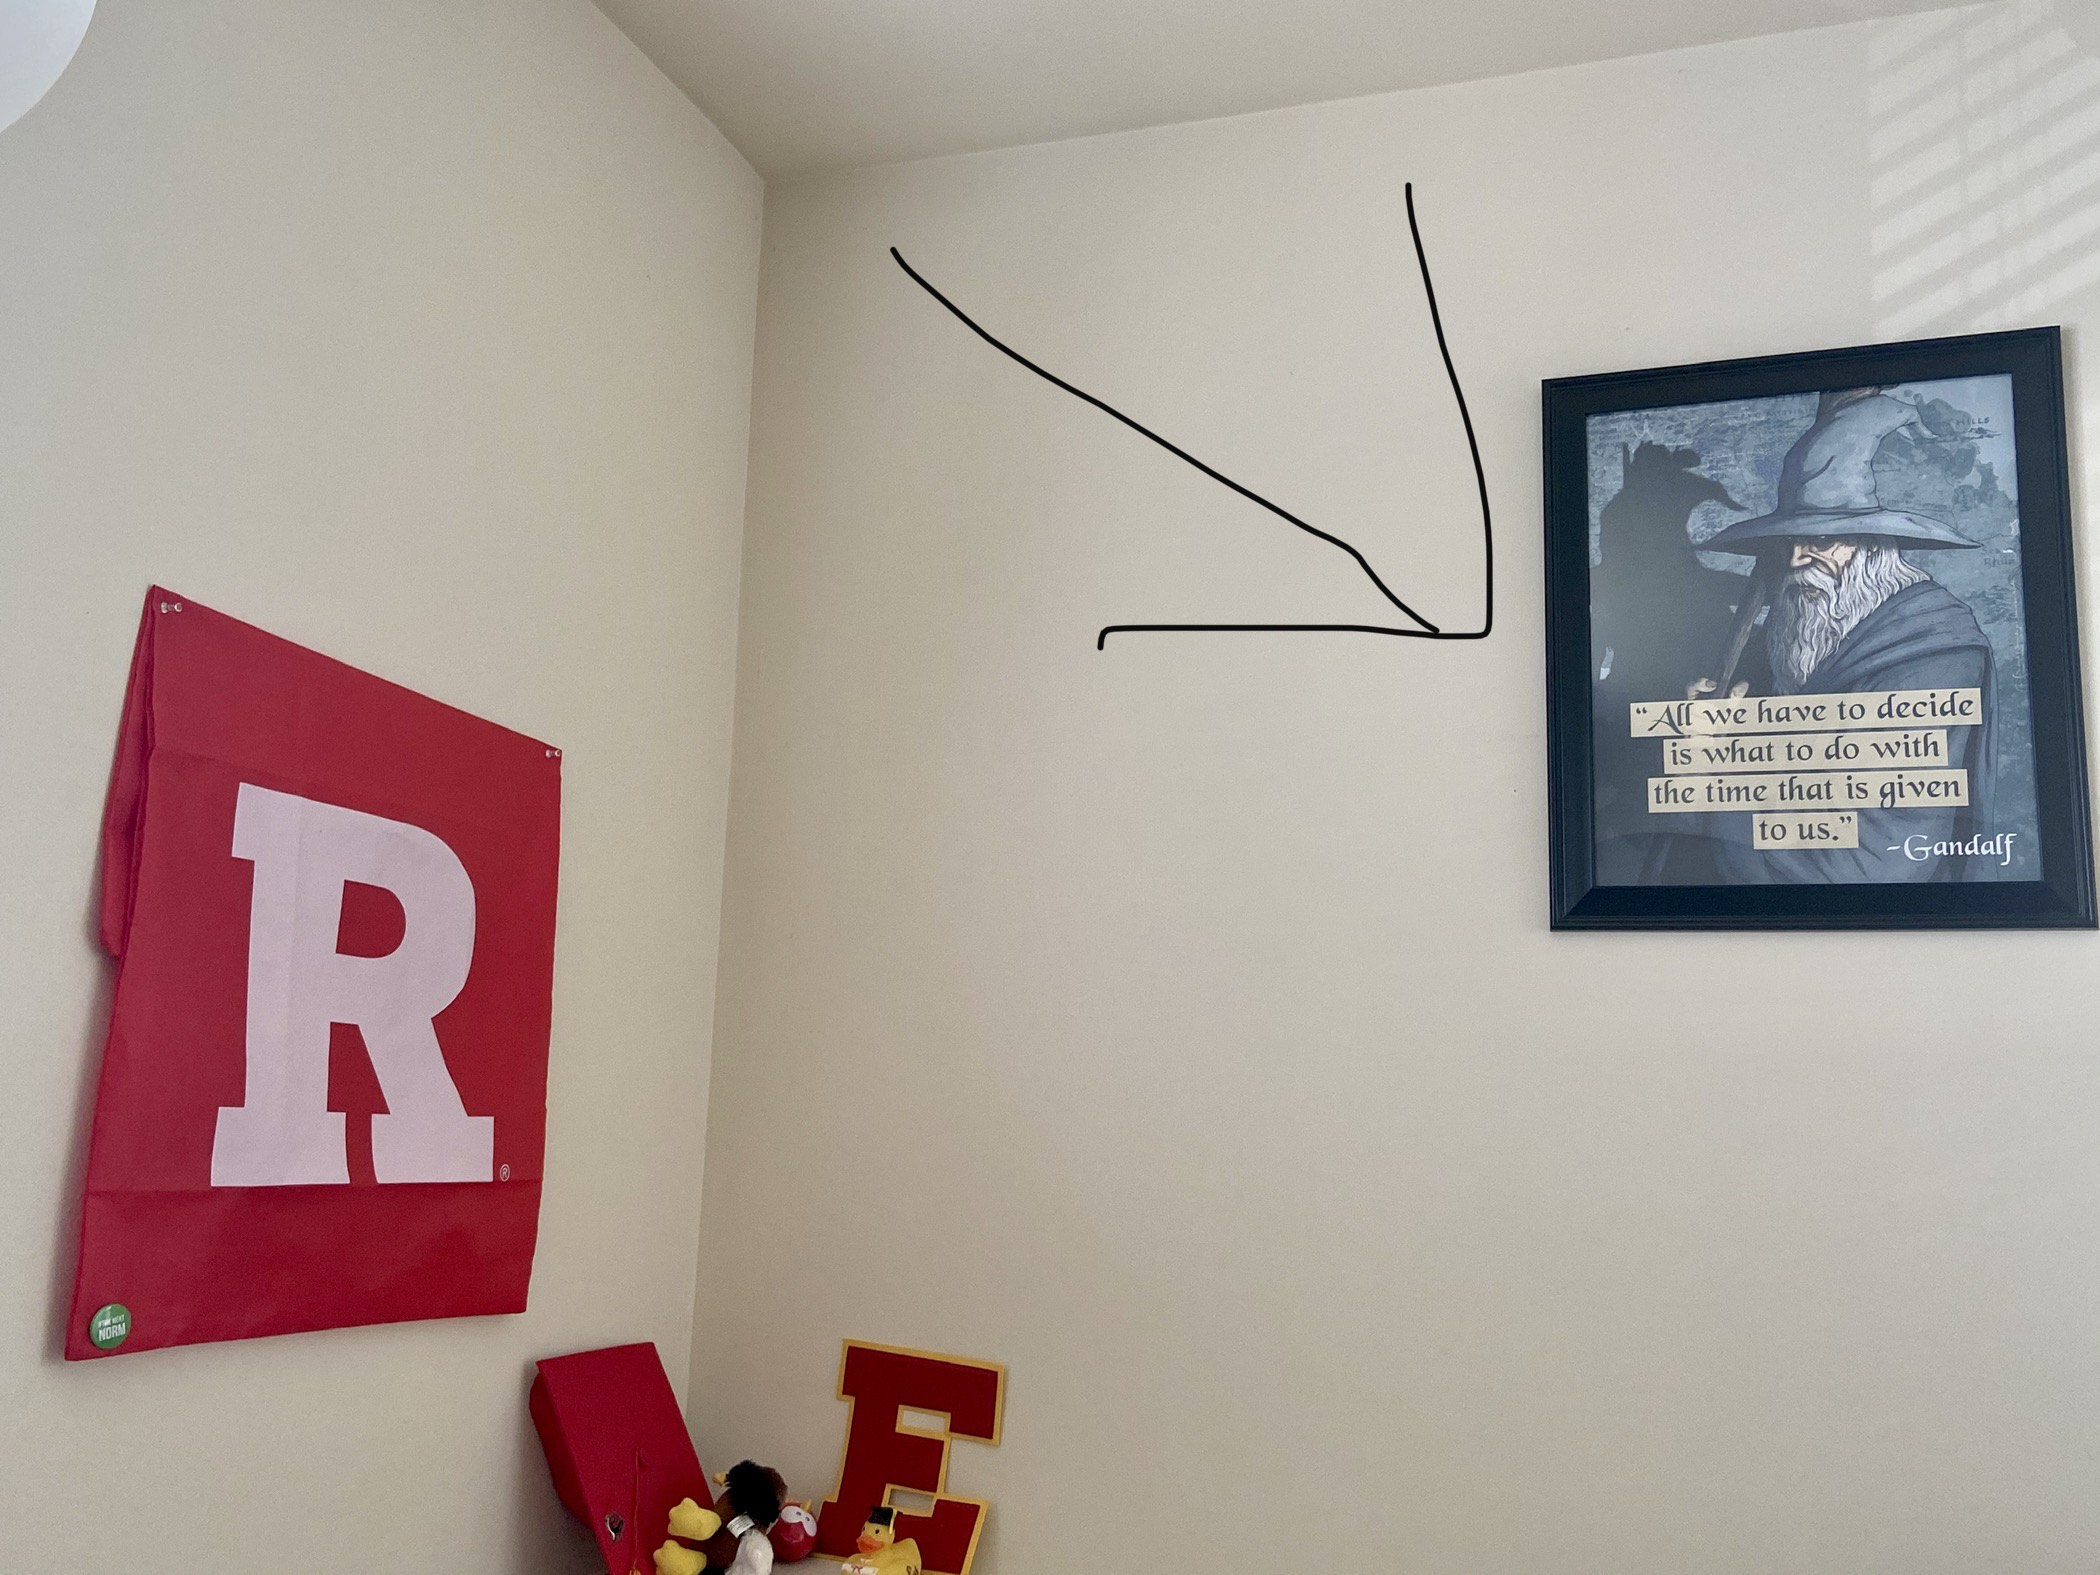
\includegraphics[width=1\textwidth]{img/JournalTwo-c8f6d4a9.png}
	\caption{My inspirational ``Gandalf'' poster!}
	\label{fig1}
\end{figure}

  \s \textit{\textbf{Dealing with Distractions}}: I miss Library of Science
  and Medicine, mostly because I can't get myself to watch a 1.5 hour movie
  in the middle of a study session in the quiet floor. Yet, that's not true in
  my current workplace. While I do try to learn more about myself and schedule
  my day accordingly, I can get it wrong, especially on Fridays. For the past
  2 weekends, I have had to work extra hours on Sunday because Friday didn't
  go so well! However, with every passing day, I get more comfortable with working
  6-7 hours a day as long as I spread my hours sufficiently.
\end{itemize}

 \item \textbf{How has research differed from your expectations?}
 \begin{itemize}
   \s \textit{\textbf{Art of Explaining}}: I did not expect that a large part
   of my research will be constantly explaining it to myself and others.
    Properly reasoning my research project is invaluable. I have experienced
   several instances of embarrasment in my meetings with my faculty
   mentor and other professors. The reason? I
   didn't think enough about my methods, forgot to review small yet significant
   details like units on a graph, assumed something was true despite lack of
   evidence, etc. I often fool myself into assuming that I understand something when I really don't.

   For example, during a presentation to a research group from the chemistry
   department, I was asked whether the subject of my talk -Variational
   Quantum Eigensolver- could solve the electronic structure problem
   \textit{within} chemical accuracy. In the context of my work, this question was a simple
   yet important one, one that I forgot to ask myself. So naturally,
   I fumbled for a few minutes. Fortunately, the leader
   of that research group saved me from further embarrasment. Whew!

   The lesson from these experiences is to be really critical when learning
   a concept or doing an experiment. Being inquisitive and transparent are
   some of the things I can do to make my explanations logically sound.
 \end{itemize}
\item \textbf{What has been your greatest success or accomplishment thus far?}
\begin{itemize}
  \s \textit{\textbf{Exciting Experiments}}: Since quantum computers can
  be efficiently accessed through IBM Cloud, I can run experiments efficiently
  and retrieve results in a matter of seconds. This means that I can go
  beyond the assertions made by research papers and actually test out the
  proposed techniques in real time. Yet, to do so, one needs to understand
  the IBM code works. This can be stressful. However, sometimes things click
  and they have done so several times this week!


  Shown below are results from an experiment testing whether I can use ``noisy''
  or error sensitive results to produce a better result i.e. a curve that
  is closer to the ideal curve. The graph below shows how it is possible to
  extrapolate from the ``noisy'' orange and green curves to produce a better
  result (red curve) which is closer to the ideal result (blue curve). The
  implications of such cheeky trick are huge: we can get somewhat accurate answers
  despite the ``noisiness'' of our current quantum devices.
  \begin{figure}[!htb]
	\centering
	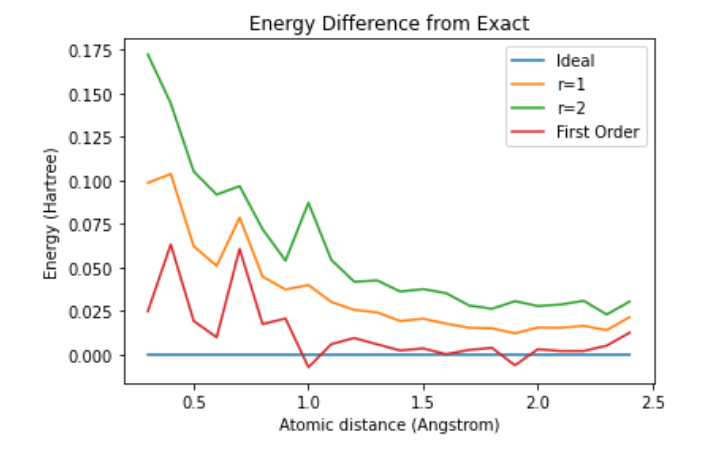
\includegraphics[width=0.95\textwidth]{img/JournalTwo-f5cc5222.png}
	\caption{Results from an extrapolation experiment on the energy dissassociation
  curves of hydrogen \(H_2\) molecule.}
	\label{}
\end{figure}
\end{itemize}
I feel proud of this result because it seemed hard to replicate when I initially read it in a paper. But having simulated such technique, I
can now investigate more complicated techniques and hopefully get to
the cutting edge, from where I can make new discoveries!

\end{itemize}

\end{document}
